\documentclass{beamer}
\usepackage{algorithm}
\usepackage[noend]{algpseudocode}
\usepackage{listings}
\usepackage{courier}
\lstset{
  language=C++,
  basicstyle=\footnotesize\ttfamily,
  numberstyle=\tiny,
  numbersep=5pt,
  tabsize=2,
  extendedchars=true,
  breaklines=true,
  %frame=b,
  keywordstyle=\color{red},
  stringstyle=\color{blue}\ttfamily,
  commentstyle=\color{greenmod},
  numberstyle=\color{violet},
  identifierstyle=\color{orange},
  showspaces=false,
  showtabs=false,
  xleftmargin=17pt,
  framexleftmargin=17pt,
  framexrightmargin=5pt,
  framexbottommargin=4pt,
  showstringspaces=false
}
\usepackage{xcolor}
\usepackage{color}
\usepackage{amsmath}

\definecolor{greenmod}{rgb}{0,0.6,0}

%% Remember: keep this PRACTICAL. How do you literally do all these things?

%% TODO:

%I'm planning on covering
%- what git is
%- why you would want to use it
%- why it might be better than other version control systems you've used before
%- some of the annoying things to watch out for
%- How to use tools like github or bitbucket to be more productive
%
%I'll probably assume that you know how to use a terminal on your
%computer and can install the git executable (on linux, it's already
%there for you, on OS X you can get it from macports or homebrew, and
%on Windows I have no idea!)
%
%If you have any more specific requests about things you're interested
%in related to git (or version control in general), let me know before
%Wednesday.
%It'll be both.
%
%For those who aren't familiar, git is a "version control" system. The
%basic functionality is being able to save and record snapshots of your
%progress with a project, so that you can always return to a working
%state. Additional features include the ability to manage different
%versions of your project ("branches") and to work on the same project
%with other people using other computers.
%
%Such a system is extremely helpful for software projects, and is
%practically essential for software projects with more than one or two
%authors. It can also be used for any set of not-too-big files: a key
%example is working on a paper in latex.
%
%Github and Bitbucket are web-based services which keep a copy of your
%project (and its history), managed with git, on their servers and give
%you lots of nice tools to interact with it.
%
%If you find yourself wasting time doing these sorts of things, git can help:
%
% - Not being able to remember which is the original version of a piece of code
%
% - Accidentally overwriting your files
%
% - Getting confused sending code around via email
%
% - Ending up with two different versions of your code and not knowing
%how to merge them
%
% - Not being able to return to a working state of your code
%
% - Not being able to quickly work with remote collaborators on code
%
% - Being slowed down by a version control system which requires
%network access at all times




% Some misc notes:
%git:

%Where it comes from (parable) 
%eWhat you can do with it
%eWhy it’s better than subversion
%e  cheap branching
%eWhat’s bad about it, and how to mitigate those factors
%e  dumb syntax
%eGUIs and web tools
%eHow to learn more
%e
%eGood habits it encourages
%e  Working on atomic units of progress
%e  Summarizing and explaining what you’re doing
%e  Making your progress visible to other people [esp. remote collaborators]
%e  Writing to be shared and extended
%e  Moving between working states
%e  Backing up remotely
%e  Maintaining a canonical version (“upstream”) of a project
%e
%eThe main objective:
%e  Overcome the energy barrier to learn and become comfortable with the tools.




%\usepackage[backend=bibtex,maxnames=100]{biblatex} %from macports texlive-bibtex-extra
%\addbibresource{PFKrylov.bib}
%\renewcommand{\footnotesize}{\tiny}


\usetheme{Madrid}
\setbeamertemplate{navigation symbols}{} % Remove the navigation symbols
\setbeamertemplate{sections/subsections in toc}[default] %Turn off ugly toc numbering
\setbeamertemplate{itemize subitem}[triangle]
\setbeamertemplate{itemize item}[triangle]
\setbeamertemplate{enumerate items}[default]
%\setbeamercovered{transparent}
\usepackage{appendixnumberbeamer}
\defbeamertemplate{section page}{customsection}[1][]{%
  \begin{centering}
    {\usebeamerfont{section name}\usebeamercolor[fg]{section name}#1}
    \vskip1em\par
    \begin{beamercolorbox}[sep=12pt,center]{part title}
      \usebeamerfont{section title}\insertsection\par
    \end{beamercolorbox}
  \end{centering}
}
\defbeamertemplate{subsection page}{customsubsection}[1][]{%
  \begin{centering}
    {\usebeamerfont{subsection name}\usebeamercolor[fg]{subsection name}#1}
    \vskip1em\par
    \begin{beamercolorbox}[sep=8pt,center,#1]{part title}
      \usebeamerfont{subsection title}\insertsubsection\par
    \end{beamercolorbox}
  \end{centering}
}
\AtBeginSection{\frame{\sectionpage}}
\AtBeginSubsection{\frame{\subsectionpage}}

%%%%%%%%%%%%%%%%%%%%%%%%%%%%%%%%%%%%%%%%%%%%%%%%%%%%%%%%%%%%%%%%%%%%%%%%%%%%%%%

\graphicspath{images/}

% clashes with beamer
%\usepackage[colorlinks=true]{hyperref}

\usepackage{booktabs}

%%%%%%%%%%%%%%%%%%%%%%%%%%%%%%%%%%%%%%%%%%%%%%%%%%%%%%%%%%%%%%%%%%%%%%%%%%%%%%%

%%%%%%%%%%%%%%%%%%%%%%%%%%%%%%%%%%%%%%%%%%%%%%%%%%%%%%%%%%%%%%%%%%%%%%%%%%%%%%%

\author{Patrick Sanan}
\institute[USI/ETHZ] 
{
USI Lugano ICS / ETH Z\"{u}rich ERDW\\
}

%%%%%%%%%%%%%%%%%%%%%%%%%%%%%%%%%%%%%%%%%%%%%%%%%%%%%%%%%%%%%%%%%%%%%%%%%%%%%%%

\title{A Git Tutorial} 
\subtitle[]{What it is, how you use it, and what it's good for}
\date[]{} 
% Long date messes up footer

%%%%%%%%%%%%%%%%%%%%%%%%%%%%%%%%%%%%%%%%%%%%%%%%%%%%%%%%%%%%%%%%%%%%%%%%%%%%%%%

\begin{document}

%%%%%%%%%%%%%%%%%%%%%%%%%%%%%%%%%%%%%%%%%%%%%%%%%%%%%%%%%%%%%%%%%%%%%%%%%%%%%%%%
%%%%%%%%%%%%%%%%%%%%%%%%%%%%%%%%%%%%%%%%%%%%%%%%%%%%%%%%%%%%%%%%%%%%%%%%%%%%%%%%

\begin{frame}[fragile]
\titlepage 
\end{frame}

%%%%%%%%%%%%%%%%%%%%%%%%%%%%%%%%%%%%%%%%%%%%%%%%%%%%%%%%%%%%%%%%%%%%%%%%%%%%%%%

\begin{frame}
\tableofcontents 
\end{frame}

\section{Who is this for?}
\begin{frame}[fragile]
\frametitle{}
Assumptions about the audience:
\begin{itemize}
\item You use code
\item You sometimes feel like you're wasting your time when you work with code, especially when it comes time to collaborate
\item You know how to use a terminal, terminal-based text editor, and login file on your computer \footnote{If not, ask me afterwards}
\item You don't care much about the inner workings of git, as long as it functions
\end{itemize}
\uncover<2>{ 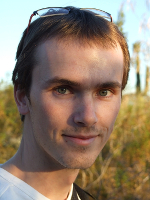
\includegraphics[width=50px]{antoine.jpg} (or you are Antoine)}
\end{frame}

% As we proceed, I will use a two examples:
%1. a toy code that we've been working with.
% 2. an extremely simple project that we'll start from scratch

% You can find all this material (tracked with git of course), at
%  bitbucket.org/psanan/gittutorial
% ?? Actually, move this to github..

\section{What is git?}
\begin{frame}[fragile]
\frametitle{Why Version Control?}
\begin{itemize}
\item
git is a \emph{Version Control System (VCS)}.
\item 
We will show how one might invent such a thing.\footnote{based on \href{http://tom.preston-werner.com/2009/05/19/the-git-parable.html}{``The Git Parable'' by Tom Preston-Werner}}
\end{itemize}
\end{frame}

\begin{frame}[fragile]
\frametitle{Tracking History - Snapshots}
\begin{itemize}
\item When working on code, it's natural want to save certain states.
\item You might do this manually, creating folders with different \emph{snapshots} of your data every once in a while.
\end{itemize}
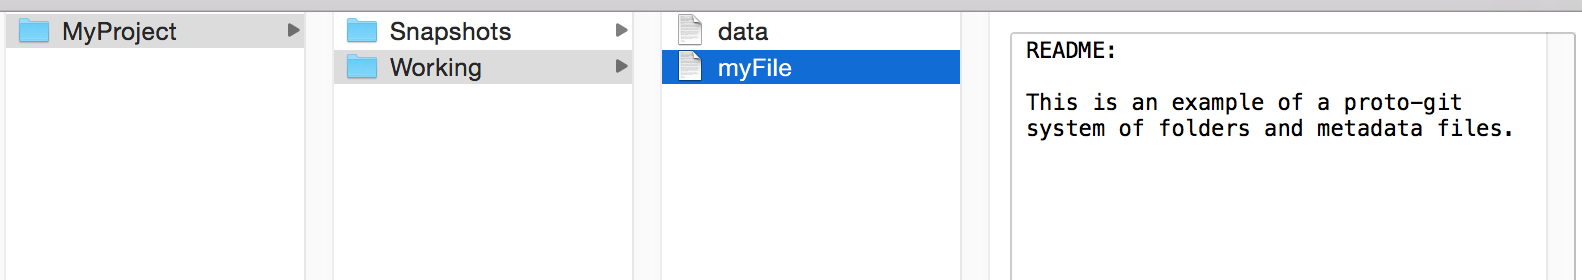
\includegraphics[scale=0.4]{snapshot1.png}\\
\vspace{10px}

\includegraphics[scale=0.4]{snapshot2.png}

\end{frame}

\begin{frame}[fragile]
\frametitle{Adding Metadata - Commits}
\begin{itemize}
\item I might decide that I want more information about each snapshot
\item I introduce data in a new folder of \emph{commits} 
\item I want to be able to ``rewind'', so I record a \emph{parent} commit for each commit (except the first)
\end{itemize}
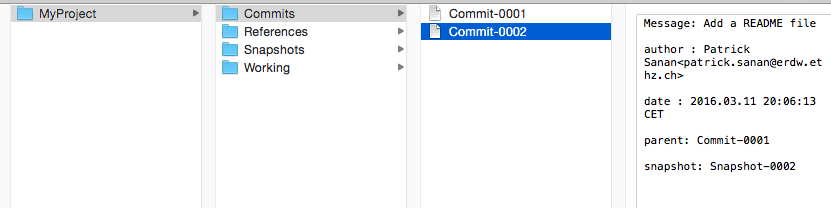
\includegraphics[scale=0.4]{commit1.png}\\
\end{frame}

\begin{frame}[fragile]
\frametitle{Adding Metadata - Commits}
\begin{itemize}
\item I also introduce a new file called \texttt{HEAD} which points to the latest commit
To save my state,
\begin{enumerate}
\item Copy the state indicated by \texttt{HEAD} to a \emph{staging area} and pick some or all of the changes from my \emph{working directory} to add there
\item Copy the staging area directory to a new snapshot
\item Create a new commit, using \texttt{HEAD} as the parent and pointing to my new snapshot
\item Update \texttt{HEAD} to the new commit
\end{enumerate}
\end{itemize}
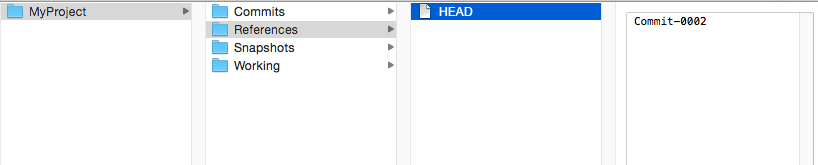
\includegraphics[scale=0.4]{commit2.png}
\end{frame}

\begin{frame}[fragile]
\frametitle{Different Versions}
\begin{itemize}
\item We can keep track of multiple version of our project by adding more \emph{references} and updating them. 
\item We change \texttt{HEAD} to now point to one of these \emph{branches}
\end{itemize}
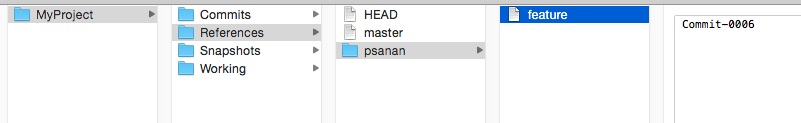
\includegraphics[scale=0.4]{branch1.png}\\
\vspace{10px}
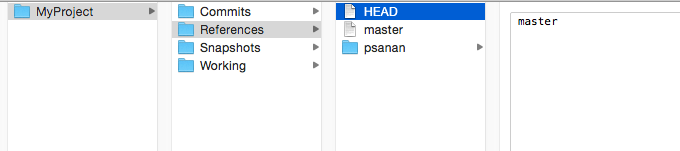
\includegraphics[scale=0.4]{branch2.png}
\end{frame}

\begin{frame}[fragile]
\frametitle{Different Versions}
\begin{itemize}
\item We realize that we can have multiple parents in a commit, which allows us to \emph{merge} branches.
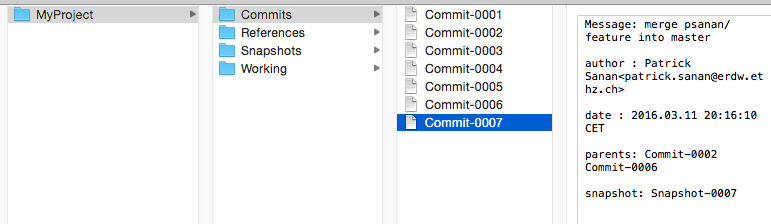
\includegraphics[scale=0.4]{branch3.png}
\end{itemize}
\end{frame}

\begin{frame}[fragile]
\frametitle{Other People}
\begin{itemize}
\item Now, suppose you and I both have a copy of this \emph{repository} and want to collaborate
\item We have the clever idea that we can name the files by applying a function\footnote{a \emph{cryptographic hash function}} to their contents. Now, if we have files with the same names, we have the same data.
\end{itemize}
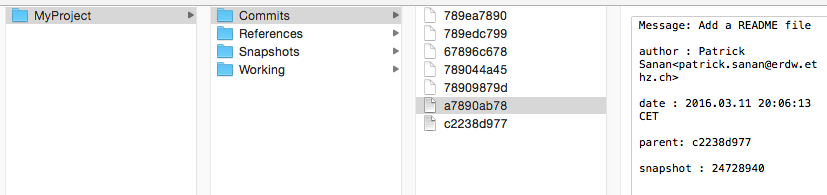
\includegraphics[scale=0.4]{remote1.png}\\
\vspace{10px}
\end{frame}

\begin{frame}[fragile]
\frametitle{Other People}
\begin{itemize}
\item I keep a special set of \emph{remote references} to branches which correspond to your repository
\item When I want your changes from a branch
\begin{itemize}
\item You send me the reference to your version of the branch.
\item I look at the reference and ask for any files (commits and snapshots) that I am missing.
\item I can make a merge commit as before. 
\item I can then send you my reference and you can repeat the steps so that we are synchronized.
\end{itemize}
\end{itemize}
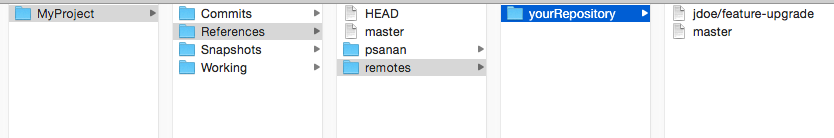
\includegraphics[scale=0.4]{remote2.png}
\vspace{10px}
\end{frame}

\begin{frame}[fragile]
\frametitle{That's it!}
Git is simply software that, at its core, does all the things we just mentioned, properly implemented:
\begin{itemize}
\item Defines data in a \emph{repository}
\item Records \emph{snapshots} of a set of files
\item Gives you a way to obtain a copy of the files, edit them, and add your changes as a new snapshot.
\item Keeps track of \emph{commits} for each snapshot: a summary, who made the changes, when, and from what previous snapshot.
\item Keeps track of pointers to commits called \emph{branches} and provides a way to increment them, as new commits are added, and a way to merge them.
\item Keeps track of references to \emph{remote repositories} and provides a way to send and recieve repository data.
\end{itemize}
\end{frame}

\begin{frame}[fragile]
\frametitle{Aside: Differences from other Version Control Systems}
Some of you may be scarred by previous version control systems.
\begin{itemize}
\item It's very easy to set up a repository and share it.
\item Git (and Mercurial/Hg) are \emph{Distributed Version Control Systems}. 
\begin{itemize}
\item There is no need to be in constant contact with a central server
\item You have a copy of everything on your machine
\item Branching is cheap
\end{itemize}
\item It's hard to lose data with git. 
\begin{itemize}
\item
You have a complete copy of the history locally. 
\item The files in the \texttt{.git} folder are all named with cryptographic hashes, so if they are corrupted, you will find out.
\end{itemize}
\end{itemize}
\end{frame}

\begin{frame}[fragile]
\frametitle{A Git Repository in Graphical Form}
\begin{itemize}
\item Git repositories are commonly drawn as ``trees'' (more precisely, Directed Acyclic Graphs (DAGs).
\item A commit is a node and edges pointing to its parent(s). 
\item A branch is a box which points to a commit
\item \texttt{HEAD} is a box which points to a branch
\item Merges are commits with exactly two parents
\item (Aside: You can also use \lstinline{git label} to add fixed references to important commits)
\end{itemize}
Let's draw one on the board..
\end{frame}

\section{How do I use it?}

\subsection{Basic Usage}
\begin{frame}[fragile]
\frametitle{Obtaining Git}
There are many ways to obtain git. 
You can download a binary from \texttt{git-scm.com}, if you are using Ubuntu, you likely already have it, and if you used MacPorts or Homebrew on OS X you can install it there.
\end{frame}

\begin{frame}[fragile]
\frametitle{Setting Git Up}
To be able to keep track of who made which changes, git needs to know who you are.
%% Setting it up. You need to tell git who you are. [crib here from Lecture 1 and from git book]
The best way to do this is to tell git these things each time you log into a terminal.
In addition to your name and email address, I recommend you turn on colors and set your favorite text editor to edit commit messages.
\begin{lstlisting}[language=]
git config --global user.name "Patrick Sanan"
git config --global user.email "patrick.sanan@erdw.ethz.ch"
git config --global color.status auto
git config --global color.branch auto 
git config --global core.editor vim
\end{lstlisting}
\end{frame}

\begin{frame}[fragile]
\frametitle{Creating a Repository}
\begin{itemize}
\item From now, we'll start working on a real example. 
\item I assume that I have a working \lstinline{git} executable and that I have set up my login file to establish my identity.
\item I create a new directory and create a new git repository there:
\begin{lstlisting}[language=C++]
mkdir myDemoProject
cd myDemoProject
git init
\end{lstlisting}
\item Data is created in the \lstinline{.git} directory. Never change anything in this directory.
\item (I'll be doing everything from the terminal here, but you can also use various GUI tools to work with git: \texttt{git-scm.com/downloads/guis})
\end{itemize}
\end{frame}

\begin{frame}[fragile]
\frametitle{Adding and Tracking changes to files}
\begin{itemize}
\item The \lstinline{git add} command moves files to the staging area.
\item \lstinline{git commit} creates a new snapshot from staging area, creates a new commit, and updates the branch reference.
\item \lstinline{git status} lets you know the current state.
\item Try the following (use your favorite editor instead of vim)
\begin{lstlisting}[language=C++]
vim data.txt
git status
git add data.txt
git status
git commit
git log
\end{lstlisting}
\end{itemize}
\end{frame}

\begin{frame}[fragile]
\frametitle{Writing Good Commit Messages}
\begin{verbatim}
Component: summary

After a blank line, describe what you did. 
This will be something read later on by you,
and by other people trying to figure out what
broke their code. If you did something that could 
cause problems for someone, note it here. It's
also a good idea to wrap the lines yourself.
\end{verbatim}
\end{frame}

\begin{frame}[fragile]
\frametitle{What's in a commit?}
\begin{itemize}
\item For basic usage, anything you changed since the last time your code worked.
\item For work in teams or on larger projects,
\begin{itemize}
\item Changes related to a particular task on a particular component
\item Something that is reasonably atomic
\item Something which won't interfere with other people's work without cause
\end{itemize}
\end{itemize}
\end{frame}

\begin{frame}[fragile]
\frametitle{Branching}
\begin{itemize}
\item By default you are on a branch called \texttt{master}
\item Create branches with \lstinline{git branch new-branch-name}
\item A good way to name branches is \lstinline{yourname/component-description}.
\item \emph{checkout} a branch with \lstinline{git checkout}. This means update \texttt{HEAD} to point to the branch, and update the working directory to the snapshot indicated by the branch.
\item Try:
\begin{lstlisting}[language=C++]
git branch psanan/data-reorganize
git checkout psanan/data-reorganize
vim data.txt
git add data.txt
git commit
git log
git checkout master
vim data.txt
git log
\end{lstlisting}
\end{itemize}
\end{frame}

\begin{frame}[fragile]
\frametitle{States of Files}
It's worth reiterating the different states that files can be in.
\begin{itemize}
\item \lstinline{git status} will tell you about the states of files
\item They can be unmodified from the current snapshot
\item They can have unstaged changes
\item They can have staged changes staged (note that you can stage parts of files)
\item They can be untracked
\item (They can be also be ignored if you defined a special \texttt{.gitignore} file)
\end{itemize}
\end{frame}


\begin{frame}[fragile]
\frametitle{The Most Important Commands}
There are many commands in git. These are some more handy ones
\begin{itemize}
\item \lstinline{git help}
\item \lstinline{git diff [filename]} (what's changed?)
\item \lstinline{git log [-10]} (see 10 commits worth of history)
\item \lstinline{git branch -avv} (see ALL branches)
\end{itemize}
\end{frame}


% Panic!! What to do if you get into trouble??
%% Relax. Most things in git are non-destructive. Exceptions: thing you have to ``force'', rebasing, hard resetting.
%% git status will often tell you how to abort something (say, a merge).


\begin{frame}[fragile]
\frametitle{For More}
The Git Book : free at \href{https://git-scm.com/book}{git-scm.com/book} \\

\includegraphics[width=100px]{progit2}
\end{frame}

\subsection{Remote Repositories and Tools}

\begin{frame}[fragile]
\frametitle{Getting a Copy of an existing project}
\begin{itemize}
\item
The most common way to start working on a git project is to make a copy of someone else's project on GitHub on BitBucket with \lstinline{git clone}
\item You only need to know the address of the repository
\begin{lstlisting}[language=C++]
git clone git@bitbucket.org:psanan/gittutorial
\end{lstlisting}
\item This creates a new local repository as a copy of the remote repository.
\item To simple obtain code with git, this is all you need to know.
\end{itemize}
\end{frame}

\begin{frame}[fragile]
\frametitle{Remote Basics (1/2)}
\begin{itemize}
\item
You can define \emph{remote} repositories with the \lstinline{git remote add <name> <address>}.
\item There are two ways to connect , HTTPS and SSH. The latter will let you use an SSH key, so opt for it when possible.
\item You can have references to branches on these repositories
\item you can tell your local branches to \emph{track} remote branches. The remote branch is defined as the \emph{upstream} branch.
\item This is set up for you with the \lstinline{master} branch when you use \lstinline{git clone} to obtain a remote repository.
\end{itemize}
\end{frame}

\begin{frame}[fragile]
\frametitle{Remote Basics (2/2)}
\begin{itemize}
\item \lstinline{git fetch updates your local copy of the remote branch corresponding to your current branch}
\item \lstinline{git pull} calls \lstinline{git fetch} and also merges the remote branch into yours.
\item \lstinline{git push} sends your local branch to be merged with the remote branch.
\item \lstinline{git push -u <remotename> <branchname>} is a shortcut to push a new branch to the remote and track it.
\end{itemize}
\end{frame}

\begin{frame}[fragile]
\frametitle{An Extremely Common Mistake}
\begin{itemize}
\item \textbf{Very Important}: You keep local copies of remote branches in your local repository. For instance, with \lstinline{git branch -a} you might see some branches like this
\begin{lstlisting}[language=C++]
$ git branch -a
 * master
   remotes/origin/HEAD -> origin/master
   remotes/origin/master
\end{lstlisting}
When you check out a branch that is tracking a remote branch, you will see something like this:
\begin{lstlisting}[language=C++]
$ git checkout master
Switched to branch 'master'
Your branch is up-to-date with 'origin/master'.
\end{lstlisting}
This does \textbf{NOT} mean that your branch is up to date with the remoter branch! It means that your branch is up to date with the local copy of that branch, named \lstinline{origin/master} here.
If you want to make sure you are really up to date, you must call \lstinline{git fetch}
\end{itemize}
\end{frame}

\begin{frame}[fragile]
\frametitle{BitBucket and GitHub}
The first important point is that the repository that GitHub or BitBucket store is the same as the one on your local machine. The only thing that makes is special is that you tell your local branches about certain ``upstream'' branches, which affect how \lstinline{git fetch}, \lstinline{git pull}, and \lstinline{git fetch} behave.

You can follow updates to a project, browse it, and make comments on the bwebsites.

GitHub and BitBucket include great documentation.
\end{frame}

\begin{frame}[fragile]
\frametitle{Setting Up An Account}
Go to GitHub or BitBucket and follow the instructions. 

It's worthwhile to set up password-free access with SSH keys\footnote{I won't cover this in detail, but ask me if you are having trouble with this}.
\href{https://confluence.atlassian.com/bitbucket/set-up-ssh-for-git-728138079.html}{https://confluence.atlassian.com/bitbucket/set-up-ssh-for-git-728138079.html}
\href{https://help.github.com/articles/adding-a-new-ssh-key-to-your-github-account/}{https://help.github.com/articles/adding-a-new-ssh-key-to-your-github-account/}

BitBucket or GitHub? You can sign up for both. For all but the most advanced users, the two services are essentially the same. 

GitHub is usually considered to be the bigger dog, with more users.

Currently, BitBucket will give you much more for free if you sign up with an academic email address.
\end{frame}

\begin{frame}[fragile]
\frametitle{Putting your Project on Github or Bitbucket}
Follow the instructions on the site.
\begin{itemize}
\item With the website interface, create a git repository on the remote server
\item Tell your local repo the address
\item Tell all your local branches to track new remote branches on this remote server
\end{itemize}

Let's do this now for our demo project.

\end{frame}

\begin{frame}[fragile]
\frametitle{To Rewrite or not to Rewrite?}
We won't go into any of the details of how to do it here, but you can rewrite your git history.

An important rule is once another person is tracking a branch, do NOT rewrite the history of that branch. 

Tension arises because git history serves two, sometimes competing, purposes:
\begin{enumerate}
\item Record history so you can go back (never rewrite!)
\item Organize code development into logical commits (rewrite!)
\end{enumerate}

A good rule is to approach the history of your personal branches with the second mentality, but 
approach shared branches with the first.

\end{frame}

\subsection{Demo: Joining a project}

\begin{frame}[fragile]
\frametitle{}
Fortunately, the workflow for joining an existing project hosted on GitHub or BitBucket is very simple!
Let's perform a typical example:
\begin{lstlisting}[language=C++]
git clone https://github.com/psanan/gittutorial-demo.git
cd gittutorial-demo
git branch psanan/helloworld
git checkout psanan/helloworld
vim hello.c
git add hello.c
vim README.md
git add README.md
git status
git commit
git push -u origin psanan/helloworld
git checkout master
vim README.md
git add README.md
git commit
git merge psanan/helloworld
git push
\end{lstlisting}
And let's take a look on GitHub
\end{frame}

\section{More selling points}
\begin{frame}[fragile]
\frametitle{Selling Points}
\begin{itemize}
\item A way to accidentally lose a lot less data
\item A handy way of dealing with code which you commonly use on multiple machines (laptop, desktop, local cluster, supercomputer)
\item A way to have a canonical version of code (on GitHub or BitBucket)
\item Some added peace of mind that your code is backed up
\item An easy way to share your project
\item An easy way to join or use other projects
\item A nice way to organize your work
\item A good way to efficiently work with remote collaborators on code (or a paper)
\end{itemize}
\end{frame}

\section{Annoyances and Solutions}
\begin{frame}[fragile]
\frametitle{How do I remember all these stupid commands?!}

\includegraphics[width=100px]{git.png}
http://xkcd.com/1597/
\begin{itemize}
\item \lstinline{git status} gives you hints
\item \lstinline{git help [command]} gives you the arbitrary command line flags
\item You can use a GUI tool if you would like. Ther is a built-in one, \lstinline{git gui}, and many other options:
\href{git-scm.com/downloads/guis}{git-scm.com/downloads/guis}
\end{itemize}

\end{frame}

% The syntax
%% People often complain (see git xkcd)

% It's a useful enough tool to justify learning: there are a few commands you will use all the time,
%  and the rest you can look up
% git status tells you a lot
% git help [function] tells you a lot
% make sure you understand the underlying models. Commits, the staging area, branches, remotes.

% A GUI tool is a useful tool, but it really helps to know the model underlying git
%  For things like commiting parts of files and reviewing your change sets, these tools are great.
% GitX, GitK, GitHub, SourceTree, git-gui ..
% Even MATLAB seems to have some git functionality these days

\begin{frame}[fragile]
\frametitle{Merging is terrible!!}

\includegraphics[width=100px]{chimera.jpg}
\end{frame}


% Merges
%% Pull often
%% Make commits on contained things

\begin{frame}[fragile]
\frametitle{Where am I?}
% Picture of an empty terminal
% turn on color

% Remember useful git commands:
\begin{itemize}
\item \lstinline{git status}
\item \lstinline{git fetch}
\item \lstinline{git log -10}
\item \lstinline{git branch -avv} (See \lstinline{git help branch} for the options)
\item \lstinline{git remote -vv}
\end{itemize}

% git prompt

% Visualize your project on github/bitbucket or with a GUI tool

\end{frame}

\begin{frame}[fragile]
\frametitle{Uncommitted changes, need to work on another branch}
\begin{itemize}
\item Make contained commits as you work. 
\item Make a new branch, commit. Assuming you are on the \texttt{master} branch,
\begin{lstlisting}[language=C++]
git branch psanan/component-experimental-feature
git add file1 file2
git commit 
git checkout master 
git pull
\end{lstlisting}
\item Stash the changes
\begin{lstlisting}[language=C++]
git stash
git checkout somebody/component-description
[.. do things ..]
git checkout master
git stash apply
\end{lstlisting}
This is obviously dangerous because you need to remember where you were. Reserve for when someone comes to your desk asking questions.
\item Throw away all your changes (\textbf{dangerous: this actually deletes data!})
\begin{lstlisting}[language=C++]
git reset --hard HEAD
\end{lstlisting}
Again, unlike everything else we've shown today, this actually destroys data.
\end{itemize}
\end{frame}

\begin{frame}[fragile]
\frametitle{}
The End. \\



\end{frame}


\end{document}
